\documentclass[12pt,a4paper]{article}
\usepackage[utf8]{inputenc}
\usepackage[turkish]{babel}
\usepackage{amsmath,amssymb,amsfonts,amsthm}
\usepackage{geometry}
\geometry{top=2.5cm,bottom=2.5cm,left=2.5cm,right=2.5cm}
\usepackage{xcolor}
\usepackage{tikz}
\usetikzlibrary{babel,arrows.meta,positioning,calc}
\usepackage{pgfplots}
\pgfplotsset{compat=1.18}
\usepackage[most]{tcolorbox}
\usepackage{hyperref}
\usepackage{caption}
\usepackage{booktabs}
\usepackage{tabularx}

% -------------------------------------------------
% style.tex – Ortak paketler ve tcolorbox tanımları
% -------------------------------------------------
\usepackage[utf8]{inputenc}
\usepackage[turkish]{babel}
\usepackage{amsmath,amssymb,amsfonts,amsthm}
\usepackage{geometry}
\geometry{top=2.5cm,bottom=2.5cm,left=2.5cm,right=2.5cm}
\usepackage{xcolor}
\usepackage{tikz,pgfplots}
\pgfplotsset{compat=1.18}
\usepackage[most]{tcolorbox}
\usepackage{hyperref}
\usepackage{caption,booktabs,tabularx}

% ---------- Renk tanımları ----------
\definecolor{purp}{RGB}{102,51,153}
\definecolor{tealblue}{RGB}{0,120,130}
\definecolor{mainblue}{RGB}{26,82,118}
\definecolor{alertred}{RGB}{180,40,40}
\definecolor{okgreen}{RGB}{34,139,34}

% ---------- Tek‑argümanlı kutular ----------
\newtcolorbox{box}[2][]{
  colback=white,
  colframe=purp,
  title={#2},
  arc=2mm,
  breakable,
  #1
}

\newtcolorbox{uyari}[1][]{
  colback=yellow!10,
  colframe=orange,
  title={Uyarı},
  arc=2mm,
  breakable,
  #1
}

% ---------- Diğer yardımcı kutular (isteğe bağlı) ----------
\newtcolorbox{ornek}[2][]{
  colback=mainblue!5!white,
  colframe=mainblue,
  title={#2},
  arc=2mm,
  breakable,
  #1
}

\newtcolorbox{odev}[2][]{
  colback=okgreen!5!white,
  colframe=okgreen,
  title={Çözümü Olmayan Ödev ve Tam Çözümü: #2},
  arc=2mm,
  breakable,
  #1
}

\newtcolorbox{tanim}[2][]{
  colback=gray!5!white,
  colframe=gray!60!black,
  title={#2},
  arc=2mm,
  breakable,
  #1
}

\newtcolorbox{sezgi}[2][]{
  colback=tealblue!5!white,
  colframe=tealblue,
  title={Sezgisel Bakış ve Basit Anlatım: #2},
  arc=2mm,
  breakable,
  #1
}

\title{\textbf{İSTATİSTİK TEORİSİ}\\[0.3em] \Large 4. Hafta Ders Notları ve Detaylı Konu Anlatımı}
\author{Ders Notları Düzenlemesi, Sezgisel Açıklamalar ve Çözümlü Analizler}
\date{}

\begin{document}
\maketitle

\begin{abstract}
Bu çalışma; İstatistik Teorisi dersinin 4. haftasında yer alan \textbf{Genelleştirilmiş Merkezi Limit Teoremleri} (Lindeberg-Feller ve Lyapunov), \textbf{Büyük Sayılar Yasası Kriterleri} (Kolmogorov ve Markov), \textbf{De Moivre - Laplace Teoremi} ve \textbf{Rastgele Değişken Dönüşümleri (Transformations)} konularını içermektedir. Ağır matematiksel koşullar sezgisel benzetmeler ve tam çözümlü örneklerle ele alınmıştır.
\end{abstract}

\hrule
\vspace{1em}

\section{Büyük Resim: 4. Haftada Ne Öğreniyoruz ve Neden?}

\begin{sezgi}{Dağılımlar Özdeş Olmadığında Ne Yaparız?}
Geçen hafta gördüğümüz klasik Merkezi Limit Teoremi değişkenlerin hem bağımsız hem de \textbf{aynı dağılıma sahip (i.i.d.)} olduğunu varsayıyordu.  
Fakat gerçek hayatta:
\begin{itemize}
    \item Topladığımız veriler farklı kaynaklardan (farklı fabrikalardan, farklı yaş gruplarından) gelebilir. Yani değişkenlerin varyansları ve ortalamaları birbirinden farklıdır!
    \item Soru şudur: \textbf{Değişkenler aynı dağılıma sahip olmasa bile toplamları yine de Normal Dağılıma ($N(0,1)$) gider mi?}
\end{itemize}
İşte 4. haftanın ilk konusu olan **Lindeberg-Feller** ve **Lyapunov** teoremleri bu soruya cevap verir: *"Evet, yeter ki içlerinden tek bir değişken devasa varyansıyla tüm sistemi domine etmesin!"*  
İkinci kısımda ise bir $X$ değişkeninden $Y = g(X)$ yeni bir değişken ürettiğimizde (örneğin $Y = X^2$), yeni olasılık yoğunluğunu nasıl bulacağımızı (\textbf{Değişken Dönüşümü}) öğreniriz.
\end{sezgi}

---

\section{Genelleştirilmiş Merkezi Limit Teoremleri}

Klasik Lindeberg-Lévy MLT'sinde $X_i$ değişkenlerinin aynı dağılıma sahip olması şarttır. Değişkenlerin dağılımları birbirinden farklı olduğunda aşağıdaki genellemeler devreye girer.

\subsection{1. Lindeberg - Feller Teoremi}

\begin{tanim}{Lindeberg - Feller Teoremi}
$X_1, X_2, \dots$ bağımsız ancak farklı dağılımlara sahip olabilen rastgele değişkenler olsun. $E(X_k) = \mu_k$ ve $V(X_k) = \sigma_k^2 < \infty$ olmak üzere:
\begin{equation}
    Y_k = X_k - \mu_k, \quad T_n = \sum_{k=1}^n Y_k, \quad s_n^2 = \sum_{k=1}^n \sigma_k^2
\end{equation}
tanımlansın. Eğer $\forall \epsilon > 0$ için \textbf{Lindeberg Koşulu}:
\begin{equation}
    \lim_{n \to \infty} \frac{1}{s_n^2} \sum_{k=1}^n E\left( Y_k^2 \, I_{\{|Y_k| \ge \epsilon s_n\}} \right) = 0
\end{equation}
sağlanıyorsa, standartlaştırılmış toplam standart normale dağılımda yakınsar:
\begin{equation}
    Z_n = \frac{T_n}{s_n} = \frac{\sum_{k=1}^n (X_k - \mu_k)}{\sqrt{\sum_{k=1}^n \sigma_k^2}} \xrightarrow{d} N(0, 1)
\end{equation}
\end{tanim}

\begin{sezgi}{Lindeberg Koşulunun Anlamı: "Aşırı Baskın Değişken Yoktur"}
$I_{\{|Y_k| \ge \epsilon s_n\}}$ bir gösterge fonksiyonudur; yani değişkenin toplam standart sapmadan ($\epsilon s_n$) daha büyük aşırı uç değerler alması durumudur.  
Lindeberg koşulu der ki: Toplam varyans ($s_n^2$) büyüdükçe, hiçbir tekil değişkenin aşırı uç sapması toplam sistemi tek başına esir alamaz; her bir değişkenin toplama etkisi sıfıra gider.
\end{sezgi}

\subsection{2. Lyapunov Koşulu}

\begin{tanim}{Lyapunov Koşulu (Daha Kolay Uygulanan Yeter Koşul)}
Lindeberg koşulundaki gösterge fonksiyonlu integrali hesaplamak çoğu zaman zordur. Lyapunov şunu göstermiştir: Eğer bir $\delta > 0$ için:
\begin{equation}
    \lim_{n \to \infty} \frac{1}{s_n^{2+\delta}} \sum_{i=1}^n E\left( |X_i - \mu_i|^{2+\delta} \right) = 0
\end{equation}
sağlanıyorsa, Lindeberg koşulu \textbf{otomatik olarak sağlanır} ve MLT geçerli olur:
\begin{equation}
    \frac{\sum_{i=1}^n (X_i - \mu_i)}{s_n} \xrightarrow{d} N(0, 1)
\end{equation}
(Pratikte genellikle $\delta = 1$ alınarak 3. momentler kontrol edilir).
\end{tanim}

\begin{uyari}
\textbf{Lyapunov Koşulunun Uygulanış Alanı (Sayfa 19):}
Notlarda Lyapunov koşulu tanımlanırken değişkenler için "iid" ifadesi kullanılmıştır. Oysa değişkenler iid olduğunda zaten 2. momentin varlığı (Lindeberg-Lévy) yeterlidir. Lyapunov koşulu, değişkenlerin \textbf{farklı dağılımlara sahip olduğu (özdeş olmayan)} bağımsız serilerde MLT'yi garanti etmek için kullanılır.
\end{uyari}

\subsubsection{İspat: Lyapunov Koşulu \texorpdfstring{$\implies$}{=>} Lindeberg Koşulu}
$|X_i - \mu_i| \ge \epsilon s_n$ bölgesinde $\frac{|X_i - \mu_i|}{\epsilon s_n} \ge 1 \implies \left(\frac{|X_i - \mu_i|}{\epsilon s_n}\right)^\delta \ge 1$ olur. Buradan:
\begin{equation}
    (X_i - \mu_i)^2 I_{\{|X_i - \mu_i| \ge \epsilon s_n\}} \le \frac{|X_i - \mu_i|^{2+\delta}}{\epsilon^\delta s_n^\delta}
\end{equation}
Toplamı alıp $s_n^2$'ye bölersek:
\begin{equation}
    \frac{1}{s_n^2} \sum_{i=1}^n E\left( (X_i - \mu_i)^2 I_{\{|X_i - \mu_i| \ge \epsilon s_n\}} \right) \le \frac{1}{\epsilon^\delta} \left( \frac{1}{s_n^{2+\delta}} \sum_{i=1}^n E\left( |X_i - \mu_i|^{2+\delta} \right) \right)
\end{equation}
Lyapunov terimi sıfıra gittiğinde sağ taraf sıfır olur; sandviç kuralından Lindeberg koşulu kanıtlanır.

---

\section{Büyük Sayılar Yasası İçin Kolmogorov ve Markov Kriterleri}

Değişkenlerin dağılımları aynı olmadığında ortalamanın kitle ortalamasına yakınsamasını test eden iki altın kriter vardır:

\begin{tanim}{Kolmogorov Kriteri (Güçlü BSY - SLLN)}
$\{X_n\}$ bağımsız rastgele değişkenler dizisi olsun. Eğer:
\begin{equation}
    \sum_{k=1}^{\infty} \frac{\sigma_k^2}{k^2} < \infty
\end{equation}
ise $\{X_n\}$ dizisi \textbf{Güçlü Büyük Sayılar Yasası (SLLN)}'nı sağlar ($\frac{1}{n}\sum (X_k - \mu_k) \xrightarrow{a.s.} 0$).
\end{tanim}

\begin{tanim}{Markov Koşulu (Zayıf BSY - WLLN)}
$\{X_n\}$ bağımsız rastgele değişkenler dizisi olsun. Eğer:
\begin{equation}
    \lim_{n \to \infty} \frac{1}{n^2} \sum_{k=1}^n \sigma_k^2 = 0
\end{equation}
ise $\{X_n\}$ dizisi \textbf{Zayıf Büyük Sayılar Yasası (WLLN)}'nı sağlar ($\frac{1}{n}\sum (X_k - \mu_k) \xrightarrow{P} 0$).
\end{tanim}

\begin{uyari}
\textbf{Sayfa 21'deki $p$-Serisi Harf Hatası:}
Notlarda $\sum_{k=1}^\infty \frac{1}{k^p}$ serisi için "$k \le 1$ ise ıraksak, $k > 1$ ise yakınsak" yazılmıştır. Değişken serinin indeksi olan $k$ değil, serinin kuvveti olan \textbf{$p$ sayısıdır}:
\begin{equation}
    \sum_{k=1}^{\infty} \frac{1}{k^p} \implies 
    \begin{cases}
        p \le 1, & \text{ıraksaktır (örneğin } p=1 \text{ harmonik seridir)} \\
        p > 1, & \text{yakınsaktır}
    \end{cases}
\end{equation}
\end{uyari}

\begin{ornek}{Örnek 1: $X_k \sim \text{Poisson}(k\lambda)$ İçin BSY İncelemesi}
$V(X_k) = \sigma_k^2 = k\lambda$ olsun.
\begin{enumerate}
    \item \textbf{Kolmogorov Kriteri:}
    \begin{equation}
        \sum_{k=1}^{\infty} \frac{\sigma_k^2}{k^2} = \sum_{k=1}^{\infty} \frac{k\lambda}{k^2} = \lambda \sum_{k=1}^{\infty} \frac{1}{k} = \infty \quad (\text{Harmonik seri ıraksak!})
    \end{equation}
    Kolmogorov kriteri sağlanmaz; Güçlü BSY garanti edilemez.

    \item \textbf{Markov Koşulu:}
    \begin{equation}
        \lim_{n \to \infty} \frac{1}{n^2} \sum_{k=1}^n k\lambda = \lim_{n \to \infty} \frac{\lambda}{n^2} \frac{n(n+1)}{2} = \frac{\lambda}{2} \neq 0
    \end{equation}
    Limit sıfır çıkmadığı için Markov koşulu da sağlanmaz.
\end{enumerate}
\end{ornek}

\begin{uyari}
\textbf{Sayfa 22'deki $\chi^2_k$ Örneğindeki Cebir Hatası:}
$Y_k \sim \chi^2_k \implies V(Y_k) = 2k$ için notta limit hesaplanırken: $\lim_{n \to \infty} \frac{2n}{n^2}\frac{n(n+1)}{2} = n+1 = \infty$ yazılmıştır.  
Doğru limit hesabı:
\begin{equation}
    \lim_{n \to \infty} \frac{1}{n^2} \sum_{k=1}^n 2k = \lim_{n \to \infty} \frac{2}{n^2} \frac{n(n+1)}{2} = \lim_{n \to \infty} \frac{n^2 + n}{n^2} = 1 \neq 0
\end{equation}
Limit sonsuz değil $1$'dir; ancak yine de $0$ olmadığından Markov koşulu sağlanmaz.
\end{uyari}

\begin{ornek}{Örnek 2: $Y \sim \text{Bernoulli}(p)$ ve $X_n = \frac{Y}{n}$ Dizisi}
$V(X_n) = \frac{pq}{n^2}$.
\begin{enumerate}
    \item \textbf{Kolmogorov:} $\sum_{k=1}^\infty \frac{\sigma_k^2}{k^2} = pq \sum_{k=1}^\infty \frac{1}{k^4} = pq \frac{\pi^4}{90} < \infty \implies$ \textbf{Güçlü BSY sağlar}.
    \item \textbf{Markov:} $\lim_{n \to \infty} \frac{1}{n^2} \sum_{k=1}^n \frac{pq}{k^2} = 0 \cdot \frac{\pi^2}{6} = 0 \implies$ \textbf{Zayıf BSY sağlar}.
\end{enumerate}
\end{ornek}

---

\section{4. Hafta Ödevi ve Eksiksiz Çözümü}

\begin{odev}{De Moivre - Laplace Teoreminin MÇF İle İspatı}
\textbf{Ödev Sorusu (Sayfa 22):} $X_1, \dots, X_n \overset{\text{i.i.d.}}{\sim} \text{Bernoulli}(p)$ ve $Y_n = \sum_{i=1}^n X_i \sim \text{Binom}(n, p)$ olsun.
\begin{equation}
    Z_n = \frac{Y_n - E(Y_n)}{\sqrt{V(Y_n)}} = \frac{Y_n - np}{\sqrt{npq}} \xrightarrow{d} N(0, 1)
\end{equation}
olduğunu Moment Çıkaran Fonksiyon (MGF) yöntemiyle gösteriniz. *(Notlarda çözümü boş bırakılmıştır).*

\bigskip
\textbf{Detaylı ve Adım Adım Çözüm:}
\begin{enumerate}
    \item Tek bir Bernoulli değişkeninin MÇF'si:
    \begin{equation}
        M_X(t) = E(e^{tX}) = p e^t + q, \quad (q = 1 - p)
    \end{equation}
    \item Bağımsız toplam $Y_n \sim \text{Binom}(n, p)$ için:
    \begin{equation}
        M_{Y_n}(t) = [M_X(t)]^n = (p e^t + q)^n
    \end{equation}
    \item Standardize edilmiş değişken $Z_n = \frac{Y_n - np}{\sqrt{npq}}$'nin MÇF'si:
    \begin{equation}
        M_{Z_n}(t) = e^{-\frac{npt}{\sqrt{npq}}} M_{Y_n}\left( \frac{t}{\sqrt{npq}} \right) = \left[ e^{-p \frac{t}{\sqrt{npq}}} \left( p e^{\frac{t}{\sqrt{npq}}} + q \right) \right]^n
    \end{equation}
    \item $u = \frac{t}{\sqrt{npq}}$ diyelim ($n \to \infty$ iken $u \to 0$). Doğal logaritmasını alalım:
    \begin{equation}
        \ln M_{Z_n}(t) = n \left[ -p u + \ln(p e^u + q) \right] = n \, g(u)
    \end{equation}
    \item $g(u) = -pu + \ln(pe^u + q)$ fonksiyonunun $u=0$'da Taylor serisini açalım:
    \begin{align}
        g(0) &= 0 \\
        g'(u) &= -p + \frac{p e^u}{p e^u + q} \implies g'(0) = -p + p = 0 \\
        g''(u) &= \frac{p e^u(p e^u + q) - p^2 e^{2u}}{(p e^u + q)^2} = \frac{pq e^u}{(p e^u + q)^2} \implies g''(0) = pq
    \end{align}
    \item Taylor formülü gereği: $g(u) = 0 + 0 \cdot u + \frac{pq}{2} u^2 + O(u^3)$.  
    $u = \frac{t}{\sqrt{npq}}$ yerine yazılırsa:
    \begin{equation}
        \ln M_{Z_n}(t) = n \left[ \frac{pq}{2} \frac{t^2}{npq} + O(n^{-3/2}) \right] = \frac{t^2}{2} + O(n^{-1/2})
    \end{equation}
    \item Limit alındığında:
    \begin{equation}
        \lim_{n \to \infty} M_{Z_n}(t) = \exp\left( \frac{t^2}{2} \right) \implies \boxed{Z_n \xrightarrow{d} N(0, 1)}
    \end{equation}
\end{enumerate}
\end{odev}

\begin{center}
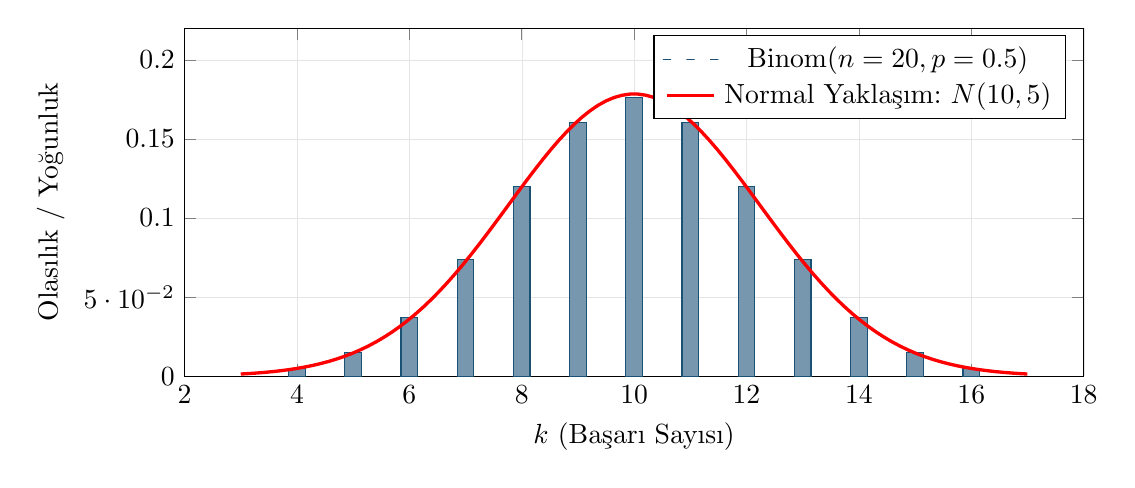
\begin{tikzpicture}
\begin{axis}[
    width=13cm, height=6cm,
    xlabel={$k$ (Başarı Sayısı)}, ylabel={Olasılık / Yoğunluk},
    xmin=2, xmax=18, ymin=0, ymax=0.22,
    grid=both, grid style={line width=.1pt, draw=gray!20}
]
    \addplot[ybar, bar width=6pt, fill=mainblue!60, draw=mainblue] coordinates {
        (4, 0.0046) (5, 0.0148) (6, 0.0370) (7, 0.0739) (8, 0.1201) (9, 0.1602)
        (10, 0.1762)
        (11, 0.1602) (12, 0.1201) (13, 0.0739) (14, 0.0370) (15, 0.0148) (16, 0.0046)
    };
    \addlegendentry{$\text{Binom}(n=20, p=0.5)$}

    \addplot[red, very thick, domain=3:17, samples=100] {
        1 / sqrt(2 * pi * 5) * exp(-(x - 10)^2 / (2 * 5))
    };
    \addlegendentry{Normal Yaklaşım: $N(10, 5)$}
\end{axis}
\end{tikzpicture}
\captionof{figure}{De Moivre-Laplace Teoremi: Binom olasılık sütunlarının kesikli yapısına rağmen Normal çan eğrisine mükemmel oturması.}
\end{center}

---

\section{Rastgele Değişkenlerde Dönüşümler (Transformations)}

\begin{sezgi}{Değişken Dönüşümü Nedir? Neden Jacobian / Türev Çarpanı Gelir?}
Bir $X$ rastgele değişkenini bir formülden geçirip yeni bir $Y = g(X)$ değişkeni elde ettiğimizde (örneğin sıcaklığı Santigrat'tan Fahrenhayt'a veya boyutu alana $Y = X^2$ çevirdiğimizde), yeni $f_Y(y)$ yoğunluğu sadece yerine koymakla bulunmaz!  
Çünkü olasılık kütlesi esner veya sıkışır. Bu esnemeyi dengelemek için diferansiyel oran olan türev çarpanı $|dx/dy|$ (Jacobian) mutlaka eklenmelidir.
\end{sezgi}

\subsection{1. Birebir ve Monoton Dönüşümler}
$X$ sürekli rastgele değişkeninin yoğunluğu $f_X(x)$ olsun. $Y = g(X)$ kesin monoton ve türevlenebilir ise:
\begin{equation}
    \boxed{f_Y(y) = f_X(g^{-1}(y)) \left| \frac{d g^{-1}(y)}{dy} \right| = f_X(x) \left| \frac{dx}{dy} \right|}
\end{equation}

\subsection{2. Birebir Olmayan Dönüşümler (\texorpdfstring{$Y = X^2$}{Y = X^2})}
$Y = X^2$ parabolik dönüşümünde hem pozitif hem de negatif $x$ değerleri aynı $y$'ye gider:
\begin{align}
    F_Y(y) &= P(X^2 \le y) = P(-\sqrt{y} \le X \le \sqrt{y}) = F_X(\sqrt{y}) - F_X(-\sqrt{y}), \quad (y > 0)
\end{align}
Türev alarak yoğunluğa geçersek:
\begin{equation}
    \boxed{f_Y(y) = \frac{1}{2\sqrt{y}} \left[ f_X(\sqrt{y}) + f_X(-\sqrt{y}) \right], \quad (y > 0)}
\end{equation}

\begin{ornek}{Örnek 3: Parçalı Yoğunluk Dönüşümü}
$X \sim \text{Uniform}(-1, 2) \implies f(x) = \frac{1}{3}, \; -1 < x < 2$ olsun. $Y = X^2$'nin yoğunluğunu bulunuz.

\bigskip
\textbf{Çözüm:}
$x \in (-1, 2)$ iken $y = x^2 \in (0, 4)$ olur. Ancak simetri bozulduğu için bölge ikiye ayrılır:
\begin{itemize}
    \item \textbf{1. Bölge ($0 < y < 1$):} Hem sol dal ($-\sqrt{y}$) hem sağ dal ($+\sqrt{y}$) mevcuttur (2 kol aktif):
    \begin{equation}
        f_Y(y) = \frac{1}{2\sqrt{y}} \left[ \frac{1}{3} + \frac{1}{3} \right] = \boxed{\frac{1}{3\sqrt{y}}}
    \end{equation}
    \item \textbf{2. Bölge ($1 \le y < 4$):} Negatif kol $-1$'de bittiği için $-\sqrt{y}$ tanım dışıdır ($f_X(-\sqrt{y})=0$). Yalnızca pozitif kol ($+\sqrt{y}$) aktiftir (Tek kol aktif):
    \begin{equation}
        f_Y(y) = \frac{1}{2\sqrt{y}} \left[ \frac{1}{3} + 0 \right] = \boxed{\frac{1}{6\sqrt{y}}}
    \end{equation}
\end{itemize}
Sonuç olarak:
\begin{equation}
    f_Y(y) = 
    \begin{cases}
        \frac{1}{3\sqrt{y}}, & 0 < y < 1 \\
        \frac{1}{6\sqrt{y}}, & 1 \le y < 4 \\
        0, & \text{diğer yerlerde}
    \end{cases}
\end{equation}
\end{ornek}

\begin{center}
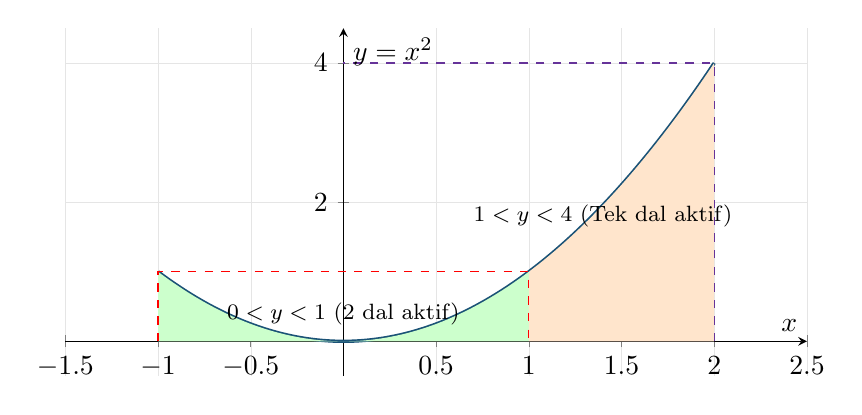
\begin{tikzpicture}
\begin{axis}[
    width=11cm, height=6cm,
    axis lines=center,
    xlabel={$x$}, ylabel={$y = x^2$},
    xmin=-1.5, xmax=2.5, ymin=-0.5, ymax=4.5,
    samples=100, domain=-1:2,
    grid=both, grid style={line width=.1pt, draw=gray!20}
]
    \addplot[mainblue, very thick, domain=-1:2] {x^2};
    \addplot[fill=green!20, draw=none, domain=-1:1] {x^2} \closedcycle;
    \addplot[fill=orange!20, draw=none, domain=1:2] {x^2} \closedcycle;

    \draw[dashed, red] (axis cs:-1,0) -- (axis cs:-1,1) -- (axis cs:1,1) -- (axis cs:1,0);
    \draw[dashed, purp] (axis cs:2,0) -- (axis cs:2,4) -- (axis cs:0,4);

    \node at (axis cs:0, 0.4) [font=\footnotesize] {$0 < y < 1$ (2 dal aktif)};
    \node at (axis cs:1.4, 1.8) [font=\footnotesize] {$1 < y < 4$ (Tek dal aktif)};
\end{axis}
\end{tikzpicture}
\captionof{figure}{$Y = X^2$ dönüşümünde $-1 < x < 2$ aralığının bölgelere ayrılması.}
\end{center}

\vspace{0.5em}
\section{4. Hafta Hızlı Tekrar ve Formül Tablosu}

\begin{table}[ht]
\centering
\small
\renewcommand{\arraystretch}{1.35}
\begin{tabularx}{\textwidth}{@{}l l X@{}}
\toprule
\textbf{Teorem / Kriter} & \textbf{Matematiksel Şart} & \textbf{Ne İşe Yarar / Anlamı} \\ \midrule
\textbf{Lindeberg Koşulu} & $\lim \frac{1}{s_n^2} \sum E(Y_k^2 I_{\{|Y_k| \ge \epsilon s_n\}}) = 0$ & Dağılımları farklı değişkenlerin toplamında MLT'yi garanti eder. \\
\textbf{Lyapunov Koşulu} & $\lim \frac{1}{s_n^{2+\delta}} \sum E(|X_k-\mu_k|^{2+\delta}) = 0$ & Lindeberg'den daha kolay hesaplanan üst moment yeter koşulu. \\
\textbf{Kolmogorov Kriteri} & $\sum_{k=1}^\infty \frac{\sigma_k^2}{k^2} < \infty$ & Farklı varyanslı bağımsız serilerde Güçlü BSY ($a.s.$) garantisi. \\
\textbf{Markov Kriteri} & $\lim_{n \to \infty} \frac{1}{n^2} \sum_{k=1}^n \sigma_k^2 = 0$ & Zayıf BSY (olasılıkta yakınsama) için pratik varyans limiti. \\
\textbf{Monoton Dönüşüm} & $f_Y(y) = f_X(x) |dx/dy|$ & Tek değişkenli birebir dönüşümde yoğunluk bulma. \\
\textbf{Karesel Dönüşüm ($X^2$)} & $f_Y(y) = \frac{1}{2\sqrt{y}}[f_X(\sqrt{y}) + f_X(-\sqrt{y})]$ & Parabolün iki kolunu birleştirerek $Y=X^2$ yoğunluğu bulma. \\ \bottomrule
\end{tabularx}
\caption{4. Haftanın Temel Teoremleri, Yakınsama Kriterleri ve Dönüşüm Kuralları}
\end{table}

\end{document}
